\documentclass[xcolor=dvipsnames]{beamer}
\useoutertheme{infolines}
\setbeamertemplate{navigation symbols}{}
\setbeamertemplate{items}[ball]
\usepackage{graphicx}
\usepackage{color}
\usepackage{xcolor}
\usepackage{verbatim}
\usepackage{float}
\setbeamertemplate{frametitle}[default][center]
\begin{document}
\title{Efficient methods for identifying mutated driver pathways in cancer}
\author{Bowen Deng}
\institute{Dept. of Prob. and Stat.}
\date{}
\begin{frame}
\maketitle
\end{frame}
\section{Introduction}
\subsection{Motivation}
\begin{frame}{Motivation}
The first step for clinical diagonostics, prognostics and targeted therapeutics of cancer is to comprehensively understand its molecular mechanisms. Large-scale cancer genomics projects are providing a large volume of data about genomic, epigenomic and gene expression aberrations in multiple cancer types. One of the remaining challenges is to \textbf{identify driver mutations, driver genes and driver pathways promoting cancer proliferation and filter out the unfunctional and passenger ones}.
\end{frame}
\subsection{Cancer's relation with genome aberrations}
\begin{frame}{Genome Aberration}
Cancer is related to genome aberrations.\\
\begin{figure}
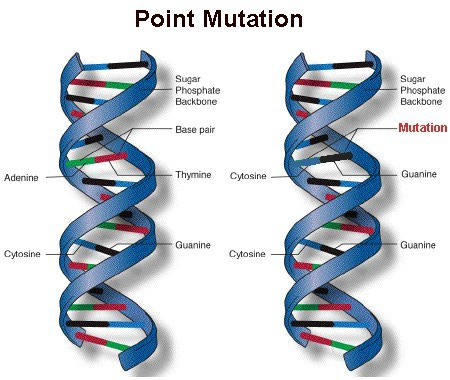
\includegraphics[width=0.45\linewidth]{genemutations.png}
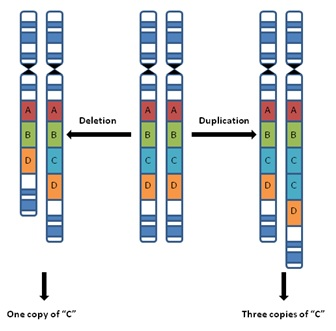
\includegraphics[width=0.45\linewidth]{cnv.png}
\end{figure}
\end{frame}
\begin{frame}{Classification of Genome Aberrations}
Genome aberrations can be classified as:
\begin{itemize}
\item Passenger Mutation: neutral to cancer proliferation\\
\item Driver Mutation: Promote cancer cell to proliferate and diffuse
\end{itemize}
Finding out driver mutation is a key to understand cancer progression, and thus aid in designing effective drugs to treat cancer.\\
\end{frame}
\subsection{Previous studies on genome aberrations}
\begin{frame}{Genome Mutation on pathway level}
The advent of high-throughput sequencing technologies enables huge number of mutation profiles.\\
Important mutations have been detected with bioinfomatics tools, but they can't capture the heterogeneity of genome aberrations.\\
And some studies found little overlap between gene mutations of two samples from the same patient.\\
We should shift the point of view from gene to pathway level.\\
\end{frame}
\begin{frame}
The problem seems unsolvable with the enormous possibility of gene combinations.\\
Yet, two blessings of the driver pathways are:\\
\begin{itemize}
\item High Coverage: many patients have at least one mutation in this pathway\\
\item High Exclusivity: most patients have no more than one mutation in this pathway\\
\end{itemize}
\begin{figure}
\centering
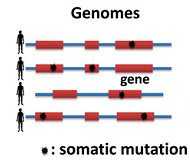
\includegraphics[width=0.4\linewidth]{segments.png}
\end{figure}
\end{frame}
\begin{frame}{Previous Pathway Studies}
Studies based on prior knowledge about pathways identify gene sets with these rules.\\
However, the knowledge about pathways is limited, and we should discover mutated driver pathways without prior knowledge.\\
Miller {\em et al.} (2011) proposed a method that identifies functional modules \textbf{without extra information}.\\
Vandin {\em et al.} (2012) introduced a novel scoring function (\textbf{maximum weight submatrix problem}) by combining coverage and exclusivity to identify the mutated driver pathway. The goal is to find efficient algorithms for the maximum weight submatrix problem. They propose a greedy algorithm and a Metropolis-Hasting algorithm for it.\\
\end{frame}
\subsection{Contributions of the paper}
\begin{frame}{Results}
In this study, we propose a BLP model equivalent to waximum weight submatrix problem and two corresponding methods:\\
\begin{itemize}
\item Exact method: Branching and Bounding algorithm\\
\item Stochastic method: Genetic algorithm\\
\end{itemize}
We also propose an integrative model that could be solved with Genetic algorithm to combine mutation and expression data. We test the methods onto simulated data and five biological datasets. The results show that our integrative model can identify more biologically relevant gene sets than one without expression data.\\
\end{frame}
\section{Materials and Methods}
\subsection{Maximum Weight Submatrix Problem}
\begin{frame}{Maximum Weight Submatrix Problem}
Given the mutation data represented by a binary mutation matrix A with m rows and n columns, the maximum weight submatrix problem is defined as finding a submatrix M of size $m\times k$ in A by maximizing the scoring function:
\[
W(M)=|\Gamma(M)|-\omega(M)=2|\Gamma(M)|-\sum_{g\in M}|\Gamma(g)|,
\]
where $\Gamma(g)$ represents the set of patients in which gene g is mutated. Thus, the first term $|\Gamma(M)|=|\cup_{g\in M}\Gamma(g)|$ is the coverage score.\\
And $\omega(M)\triangleq \sum_{g\in M}|\Gamma(g)|-|\Gamma(M)|$ measures the coverage overlap of M.\\
\end{frame}
\begin{frame}
We want to solve the following NP-hard problem:\\
\textbf{Maximum Weight Submatrix Problem (MWSP):} Given an $m \times n$ mutation matrix A and an integer $k > 0$, find the $m \times k$ column submatrix $\hat{M}$ of A that maximizes W(M).\\
\begin{figure}
\centering
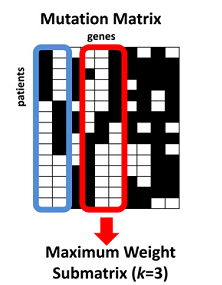
\includegraphics[width=0.4\linewidth]{mat.png}
\end{figure}
\end{frame}
\begin{frame}
The precursors have proposed a greedy algorithm and a Metropolis-Hasting algorithm to resolve the WMSP. But we would like to propose a BLP model equivalent to WMSP and apply BB algorithm and GA.
\end{frame}
\begin{comment}
\subsection{Previous algorithms}
\begin{frame}
We first review the methods proposed in Vandin {\em et al.}\\
A straightforward greedy algorithm for the MWSP is to start with the best pair $M'$ of genes and then to iteratively build the set $M$ by adding the best gene (the one that maximize $W(M)$) until $M$ has $k$ genes.\\
However, the consistency of greedy algorithm is only assured under the so-called Gene Independence Model, which is reasonable for somatic mutations (e.g., single-nucleotide mutations) but not others (e.g., copy-number aberrations).\\
\end{frame}
\begin{frame}
To circumvent the limitations of the greedy algorithm, we use a Metropolis-Hasting algorithm that does not require strict assumptions.\\
We initially select arbitrarily $k$ genes, and substitue one of the genes with an outsider with probability related to their influence on the score. The consistency is assured by MC theory. But it might stuck in a local maxima.\\
\begin{figure}
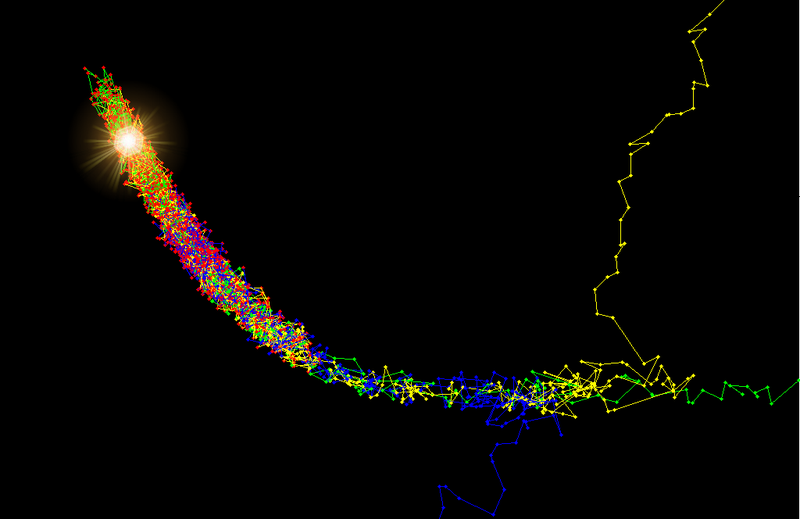
\includegraphics[width=0.45\linewidth]{MC.png}
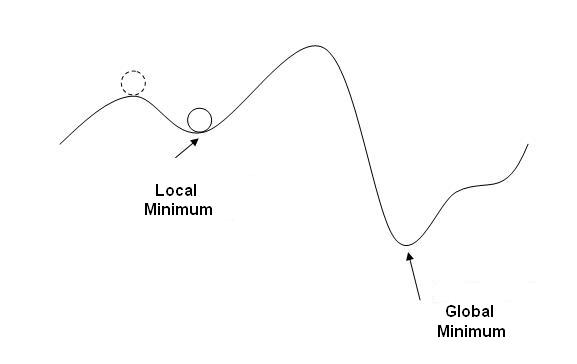
\includegraphics[width=0.45\linewidth]{trapped.png}
\end{figure}
\end{frame}
\end{comment}
\subsection{BLP model}
\begin{frame}
We can formulate the original maximum weight submatrix problem into the following optimization problem:\\
\begin{eqnarray}
\max F(x,y)=2\sum_{i=1}^my_i-\sum_{j=1}^n(x_j\cdot\sum_{i=1}^ma_{ij})\nonumber\\
s.t.
\left\{
\begin{array}{c}
\sum_{j=1}^na_{ij}x_j\geqslant y_i, i=1,\cdots,m\\
\sum_{j=1}^nx_j=k,\\
y_i,x_j\in\{0,1\},i=1,\cdots,m,j=1,\cdots,n.
\end{array}
\right.\nonumber
\end{eqnarray}
where $x_j$ is the indicator whether column $j$ of $A$ falls into the submatrix $M$, $y_i$ is the indicator whether the entries of row $i$ of $M$ are not all zeros.\\
Although the problem is NP-hard, this model can always be solved by a branch-and-bound algorithm efficiently.\\
\end{frame}
\subsection{GA: a stochastic method}
\begin{frame}
Other criteria can be designed to achieve the similar goal, and the BLP model may not be applicable to other new scoring functions. Therefore, we further design a GA.\\
The GA is a flexible and powerful technique that can be employed to optimize broad ranges of scoring functions. It has a natural connection with the current problem in terms of 'gene' and 'mutation'. It simulates the genetic variation in a population, and its evolution obeys a random selection mechanism. Moreover, it doesn't need to enumerate all the feasible solutions.\\
\end{frame}
\begin{frame}
A new model is based on such an observation that the genes in the same pathway usually collaborate with each other to execute one function.\\
Therefore, the expression profiles of gene pairs in the same pathway usually have higher correlations than that in different pathways.\\
By combining the gene expression data with the earlier problem, we define the following new measure:
\[
F_{ME}=W(M)+\lambda R(E_M)
\]
Although the maximization of $F_{ME}$ can be formulated into a binary quadratic programming problem, it is limited by the computational complexity. Here we adopt the GA framework to solve it similarly.\\
\end{frame}
\section{Results}
\subsection{Simulation study}
\begin{frame}{Simulation Study}
With simulated mutation data, we have compared the time cost of BLP, GA and MCMC on resolving the MWSP.\\
The sample number of simulation data is fixed as 500, which is larger than all our applications. The result of MCMC is obtained based on default parameters. Surprisingly, we can see that our BLP method can get the optimal solution in much shorter time than that of the MCMC. We can also observe that the GA is even faster than MCMC with n less than about 5000, which is larger than our all real applications in the following part.\\
\end{frame}
\begin{frame}
\begin{figure}
\centering
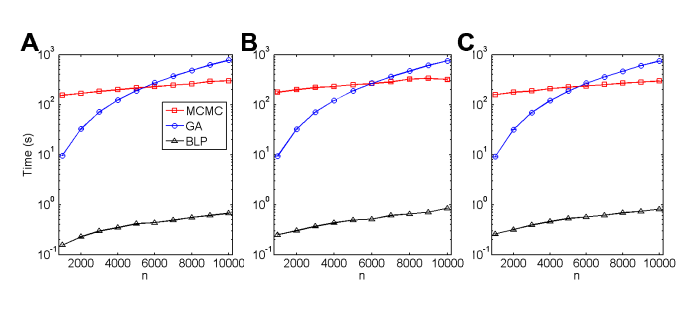
\includegraphics[width=0.8\linewidth]{comparison.png}
\end{figure}
In sum, GA method has competitive efficiency with MCMC, while our exact BLP method can work in a significantly shorter time than others, which enables it to be more applicable to real data.\\
\end{frame}
\begin{frame}
From the formulation of BLP model, we can intuitively deduce that the BLP model becomes more and more computationally costly as the sample number increases. This conjecture was confirmed by the simulation data test.\\
\begin{figure}
\centering
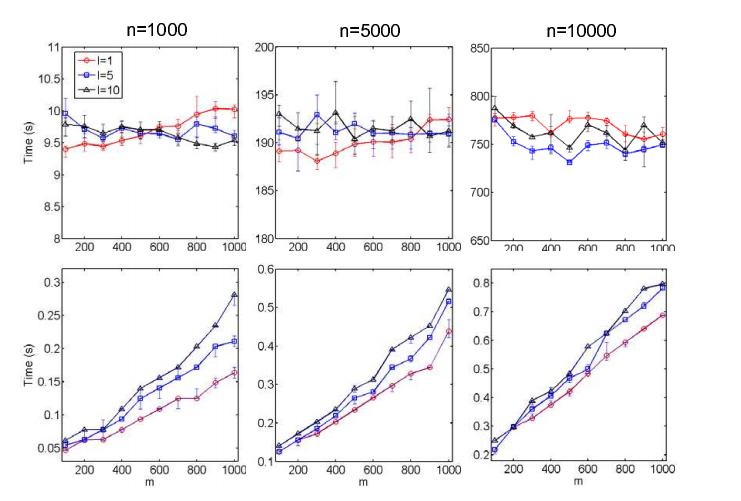
\includegraphics[width=0.8\linewidth]{GABLP.png}
\end{figure}
\end{frame}
\begin{frame}
We also test the effectiveness of GA on detecting the gene set by maximizing the integrative measure $F_{ME}$. We study the accuracy and complexity of GA on maximizing the integrative measure.\\
\begin{figure}
\centering
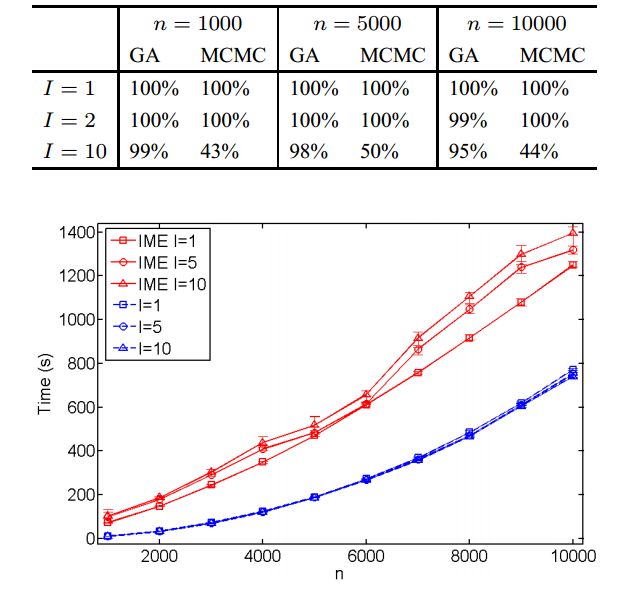
\includegraphics[width=0.6\linewidth]{table.png}
\end{figure}
\end{frame}
\subsection{Biological applications}
\begin{frame}{Applications on Biological Datasets}
We have applied out methods onto five datasets and compared their performance with MCMC. For the data used by Vandin {\em et al.} (2012), \textbf{BLP can run in a more efficient manner than MCMC and GA, while GA method also has acceptable performance.} For example, all the three methods can lead to the same gene set (EGFR, KRAS, STK11) in lung adenocarcinoma dataset with $k=3$.\\
\end{frame}
\begin{frame}{\em Head and neck squamous cell carcinoma}
The analysis result of previous study indicates that the mutations of all CDKN2A, NOTCH1, TP63 and SYNE1 function in the terminal differentiation in squamous epithelia directly or indirectly. And the set of these four genes is one suboptimal solution with $k=4$.\\
\textbf{The performance of all the algorithms are good.}
\end{frame}
\begin{frame}{\em Glioblastoma}
We first detect the mutation pattern depending on the mutation matrix only. When $k=2$, we get two optimal gene sets. After analysis of expression data, we found that the correlation between CKD4 and CDKN2B is stronger than that between TSPAN31 and CDKN2B.\\
\textbf{Involvement of expression data can discriminate the genes within identical mutation profiles and detect the one with the most relevant functional relationship.}
\end{frame}
\begin{frame}{\em Ovarian carcinoma}
We remove the five significant genes and when $k=4$, the optimal solution is KRAS, PPP2R2A, PRPF6 and TYR2. But the integrative model gets its optimal four genes that is one of the suboptimal solution of the original model. These genes show more functional relationship according to literatures. \textbf{The integrative model can detect the gene set that has a suboptimal score but more relevant function relationship}.
\end{frame}
\section{Discussion and Conclusions}
\subsection{Summary}
\begin{frame}{Summary}
In this article, the authors presented two methods to deal with wmsp proposed by Vandin {\em et al}. They first translate the problem to a BLP model and solve the model with BB algorithm and GA.\\
Moreover, they present an integrative model with expression data involved. And the model could be solved both by MCMC in Vandin {\em et al}. and GA.\\
The result was satisfactory:
\begin{itemize}
\item BLP can run in a more efficient manner than MCMC and GA, while GA method also has acceptable performance.\\
\item Involvement of expression data can discriminate the genes within identical mutation profiles and detect the one with the most relevant functional relationship.\\
    \item The integrative model can detect the gene set that has a suboptimal score but more relevant function relationship.\\
    \end{itemize}
\end{frame}
\subsection{My Ideas}
\begin{frame}{KMC algorithm}
For the original MCMC method in Vandin {\em et al.}, Metropolis-Hasting algorithm was applied. However, Metropolis algorithm might stuck at a local state for a long time. Therefore, I would like to implement an improvement of Metropolis algorithm called Kinetic Monte Carlo Algorithm (KMC) to avoid the deficiency.\\
\end{frame}
\begin{frame}{Model Revision}
For the model, I think we could focus on the patient's perspective, that each patient should ideally has one mutations in the driver pathways we select. And we can score by rows with a scoring function. If we would like to penalize more on a patient who has no mutations in the selected pathway, but less on a patient with too many mutations in the pathway, we could use a concave score. The users could adapt this penalty according to their needs.\\
The difference to the previous model is that the model is flexible with a functional control. But with small $k$, the degrees of freedom are just multivariate tuning parameters.\\
This is inspired by the natural thoughts that we could add a tuning parameter $\theta>0$ on MWSP:
\[
W(M)=|\Gamma(M)|-\theta \omega(M).
\]
\end{frame}
\begin{frame}{Weighted Sum of Row Scores}
Mathematically, we want to solve the following problem:\\
Maximum Weighted Sum of Row Scores Problem (MaWeSRoS): For an adjustable scoring function $s(x),x\in \mathbb{Z}^+\cup \{0\}$, and assuming $s$ gets its maximum at $x=1$,  we want to find an $m\times k$ submatrix $M$ in $m\times n$ mutation matrix $A$, such that it maximize the scoring function:
\[
S(M)=\sum_{i=1}^nw_is(r_i)
\]
where $r_i$ is the $i-th$ row sum in $M$, $w_i$ is the weight of the $i-th$ row, we take $w_i$ be the sum of the $i-th$ row.\\
\end{frame}
\begin{frame}{BLP Equivalence}
My model could be considered as the following BLP model:
\begin{eqnarray}
\max F(x)=2\sum_{i=1}^mw_is(\sum_{j=1}^nx_ja_{ij})\nonumber\\
s.t.
\left\{
\begin{array}{c}
\sum_{j=1}^nx_j=k,\\
x_i\in\{0,1\},i=1,\cdots,n.
\end{array}
\right.\nonumber
\end{eqnarray}
where $x_j$ is the indicator whether column $j$ of $A$ falls into the submatrix $M$, $y_i$ is the indicator whether the entries of row $i$ of $M$ are not all zeros.\\
\end{frame}
\begin{frame}{Relation with MWSP}
Moreover, MaWeSRoS is compatible for the integrative model in the paper. Just consider maximization of
\[
S(M)+\lambda R(E_M).
\]
For convenience, we can set $s(x)=1-p(|x-1|)$, where $p(\cdot)$ is an nonnegative penalty function defined on $n=0,1,\cdots$.\\
For the original MWSP, $p(x)=|x|$, so MaWeSRoS has included the original MWSP.\\
\end{frame}
\begin{frame}{Different Scores}
And for more, I can adjust the penalty function: $p_1(x)=\sqrt{x}$ for more emphasis on coverage, $p_2(x)=x^2$ for more emphasis on exclusivity, $p_3(x)=I(x>0)$ for same penalty on non-one row sums, $p_4(x)=0$ for homogeneous penalty (no penalty on overlapping). We can also set asymmetric, e.g. $s_1(x)=I(x\leqslant1)$ or $s_2(x)=I(x\geqslant1)$, according to our need and emphasis.\\
\begin{figure}
\centering
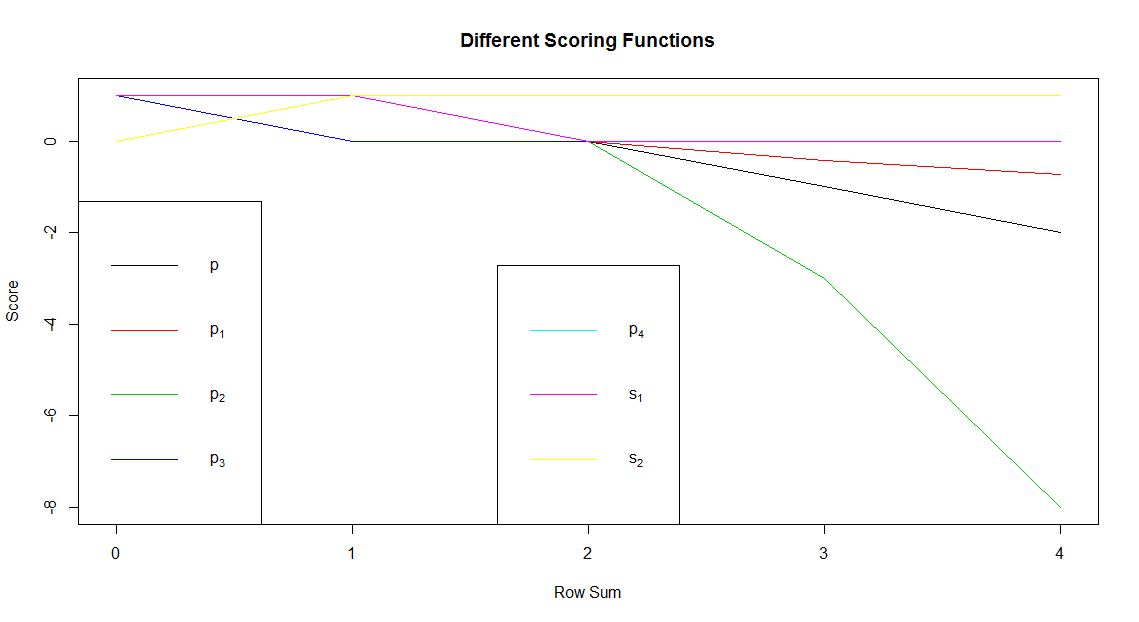
\includegraphics[width=0.8\linewidth]{diffscores.png}
\end{figure}
\end{frame}
\begin{frame}
Under this framework, the difficulty of the original BLP problem could be understood. $s(x)=1-|x-1|$ has a sharp point at $x=1$, thus it needs other constraints to describe $s(0)$, doubling the variables. Therefore, we could use square penalty, but the problem is also expensive since it is a quadratic programming (QP) problem. And square root penalty will make it harder.\\
Therefore, a general algorithm concerning this model is in need and it is not easy.\\
\end{frame}
\begin{comment}
\begin{frame}{Results}
For simplicity, we consider a $10\times 20$ mutation matrix, and take $k=5$. We use brute force algorithm for both WMSP and our model to find the optimal solution of both models.\\
For sparse matrix and small $k$, the results are almost same as MWSP results as each patient has little mutations.\\
\end{frame}
\end{comment}
\end{document}
